\documentclass[a4paper,12pt]{article}
\usepackage[utf8]{inputenc}
\usepackage{amsmath}
\usepackage{amssymb}
\usepackage{amsthm}
\usepackage{geometry}
\usepackage{graphicx}
\usepackage[hidelinks]{hyperref}
\usepackage{listings}
\usepackage{xcolor}
\usepackage{enumitem}
\usepackage{booktabs}
\usepackage[protrusion=true,expansion=false]{microtype}
\usepackage{natbib}
\usepackage{url}
\usepackage{array}
\usepackage{multirow}

\geometry{
  a4paper,
  left=2.5cm, right=2.5cm,
  top=2.5cm,  bottom=2.5cm
}

\renewcommand{\contentsname}{Inhaltsverzeichnis}
\renewcommand{\listfigurename}{Abbildungsverzeichnis}
\renewcommand{\listtablename}{Tabellenverzeichnis}
\renewcommand{\refname}{Literaturverzeichnis}
\renewcommand{\bibname}{Literaturverzeichnis}
\renewcommand{\figurename}{Abbildung}
\renewcommand{\tablename}{Tabelle}
\renewcommand{\abstractname}{Zusammenfassung}
\renewcommand{\appendixname}{Anhang}
\renewcommand{\proofname}{Beweis}
\sloppy
\emergencystretch=2em

\theoremstyle{definition}
\newtheorem{definition}{Definition}[section]
\newtheorem{beispiel}{Beispiel}[section]
\newtheorem{satz}{Satz}[section]
\newtheorem{lemma}{Lemma}[section]
\newtheorem{korollar}{Korollar}[section]
\newtheorem{bemerkung}{Bemerkung}[section]
\newtheorem{proposition}{Proposition}[section]

\setlist[itemize,1]{label=-}

\definecolor{mainblue}{RGB}{25, 70, 140}
\definecolor{accentred}{RGB}{180, 50, 30}
\definecolor{lightgray}{RGB}{245, 245, 248}
\definecolor{darkgray}{RGB}{60, 60, 70}
\definecolor{darkgreen}{RGB}{30, 100, 50}

\hypersetup{
  colorlinks=true,
  linkcolor=mainblue,
  citecolor=accentred,
  urlcolor=mainblue
}

\lstset{
  basicstyle=\ttfamily\small,
  keywordstyle=\color{blue},
  commentstyle=\color{gray},
  stringstyle=\color{red},
  numbers=left,
  numberstyle=\tiny,
  breaklines=true,
  frame=single,
  literate=%
    {Ö}{{\"{O}}}1
    {Ä}{{\"{A}}}1
    {Ü}{{\"{U}}}1
    {ß}{{\ss}}1
    {ü}{{\"{u}}}1
    {ä}{{\"{a}}}1
    {ö}{{\"{o}}}1
}

\title{\textbf{Punktwolkenverarbeitung via Subgraph Algorithmus:\\
LiDAR-basierte Objekterkennung, Registrierung und Segmentierung\\
durch graphentheoretische Signaturanalyse}}
\author{Stephan Epp}
\date{9. Juni 2026}

\begin{document}

\maketitle
\tableofcontents
\newpage

% =============================================================================
\section{Einführung}
% =============================================================================

Die \emph{Punktwolkenverarbeitung} (engl.\ \emph{Point Cloud Processing})
ist ein zentrales Problem der modernen Robotik, der autonomen Fahrzeugsysteme
und der industriellen 3D-Messtechnik. LiDAR-Sensoren (Light Detection and
Ranging) erzeugen pro Sekunde bis zu $10^6$ dreidimensionale Messpunkte,
die als \emph{Punktwolke} $\mathcal{P} = \{p_1, p_2, \ldots, p_N\} \subset
\mathbb{R}^3$ repräsentiert werden. Die effiziente Verarbeitung dieser
Rohdaten für Aufgaben wie Objekterkennung, Scan-zu-Scan-Registrierung und
semantische Segmentierung stellt hohe Anforderungen an die algorithmische
Grundlage hinsichtlich Korrektheit, Komplexität und Robustheit.

Klassische Verfahren leiden unter bekannten Schwächen: Der
\emph{Iterative Closest Point}-Algorithmus (ICP) \citep{Besl1992}
konvergiert nur bei guter Initialisierung und findet lediglich lokale
Minima. PointNet \citep{Qi2017} ist auf großen Trainingsdatensätzen
angewiesen und bietet keine formalen Korrektheitsgarantien.
Deskriptorbasierte Methoden wie FPFH \citep{Rusu2009} sind robust, aber
ohne theoretische Fundierung bezüglich struktureller Invarianzen.

Der \emph{Subgraph Algorithmus} \citep{Epp2026} bietet eine neuartige
algebraische Grundlage: Durch Signatur-Arrays und zyklische Rotationen
wird Subgraph-Isomorphie in $\Theta(n^3)$ entschieden --- optimal unter
der Strong Exponential Time Hypothesis (SETH). Die zentrale These dieser
Arbeit lautet:

\begin{quote}
  \emph{Die graphentheoretische Signaturrepräsentation des Subgraph
  Algorithmus ist eine natürliche, effiziente und formal korrekte
  Grundlage für alle drei zentralen Aufgaben der
  LiDAR-Punktwolkenverarbeitung.}
\end{quote}

\subsection{Beiträge dieser Arbeit}

Die vorliegende Arbeit leistet folgende Beiträge:
\begin{enumerate}
  \item \textbf{Graphkonstruktion:} Formaler Nachweis, dass der
        $k$-NN-Graph einer Punktwolke unter Starrköperbewegungen
        isomorph bleibt (Lemma~\ref{lem:knn_properties}).
  \item \textbf{Objekterkennung:} Reduktion des LiDAR-Erkennungsproblems
        auf Subgraph-Isomorphie mit Korrektheits- und Vollständigkeitsbeweis
        (Satz~\ref{satz:erkennung_korrektheit},
        Satz~\ref{satz:vollstaendigkeit}).
  \item \textbf{Registrierung:} Globaler Registrierungsalgorithmus über
        maximale LCS-Signaturausrichtung mit Fehlerschranke
        $|\hat\theta - \theta| \leq \pi/n$
        (Satz~\ref{satz:reg_konsistenz}, Korollar~\ref{kor:reg_fehler}).
  \item \textbf{Segmentierung:} Subgraph-Signaturklassifikator mit
        formaler Korrektheitsbedingung
        (Satz~\ref{satz:segmentierung}).
  \item \textbf{Komplexitätsanalyse:} SETH-Optimalitätsnachweis und
        Vergleich mit ICP, FPFH, PointNet
        (Satz~\ref{satz:seth}, Tabelle~\ref{tab:komplexitaet}).
\end{enumerate}

Alle Ergebnisse werden formal bewiesen und durch sieben
Matplotlib-Abbildungen illustriert.

% =============================================================================
\section{Mathematische Grundlagen}
% =============================================================================

\subsection{Punktwolken und metrische Struktur}

\begin{definition}[LiDAR-Punktwolke]
  \label{def:punktwolke}
  Eine \emph{LiDAR-Punktwolke} ist eine endliche Menge
  $\mathcal{P} = \{p_1, \ldots, p_N\} \subset \mathbb{R}^3$,
  wobei jedem Punkt $p_i = (x_i, y_i, z_i)^{\mathrm{T}}$ eine
  Reflexionsintensität $r_i \in [0,1]$ zugeordnet sein kann.
  Die \emph{paarweise Distanzmatrix} ist
  $D \in \mathbb{R}^{N \times N}$ mit $D_{ij} = \|p_i - p_j\|_2$.
\end{definition}

\begin{definition}[$k$-NN-Graph einer Punktwolke]
  \label{def:knn_graph}
  Sei $\mathcal{P} = \{p_1, \ldots, p_N\}$ eine Punktwolke und
  $k \in \mathbb{N}$. Der \emph{$k$-nächste-Nachbarn-Graph} ist
  $G_\mathcal{P} = (V, E)$ mit $V = \{v_1, \ldots, v_N\}$ und
  \[
    E = \bigl\{(v_i, v_j) \;\big|\;
        p_j \in \mathrm{kNN}_k(p_i) \text{ oder }
        p_i \in \mathrm{kNN}_k(p_j)\bigr\},
  \]
  wobei $\mathrm{kNN}_k(p_i)$ die $k$ euklidisch nächsten Nachbarn
  von $p_i$ bezeichnet.
\end{definition}

\begin{definition}[Starrköpertransformation]
  \label{def:starr}
  Eine \emph{Starrköpertransformation} ist eine Abbildung
  $T_{R,t}: \mathbb{R}^3 \to \mathbb{R}^3,\; p \mapsto Rp + t$
  mit $R \in SO(3)$ und $t \in \mathbb{R}^3$.
  Sie erhält alle paarweisen Abstände:
  $\|T_{R,t}(p_i) - T_{R,t}(p_j)\| = \|p_i - p_j\|$ für alle $i,j$.
\end{definition}

\begin{lemma}[Eigenschaften des $k$-NN-Graphen]
  \label{lem:knn_properties}
  Der $k$-NN-Graph $G_\mathcal{P}$ erfüllt:
  \begin{enumerate}
    \item $|E| \leq k \cdot N$ (Kantenanzahl linear in $N$).
    \item $G_\mathcal{P}$ ist zusammenhängend für $k \geq
          \lceil \log N \rceil$, sofern $\mathcal{P}$ keine
          isolierten Teilmengen besitzt.
    \item Für jede Starrköpertransformation $T_{R,t}$ gilt:
          $G_{T_{R,t}(\mathcal{P})} \cong G_\mathcal{P}$
          (Isomorphie).
  \end{enumerate}
\end{lemma}

\begin{proof}
  \emph{(i)} Jeder Knoten $v_i$ hat höchstens $k$ ausgehende Kanten,
  also $|E| \leq k \cdot N$.

  \emph{(ii)} Für $k \geq \lceil \log N \rceil$ ist die
  Verbindungswahrscheinlichkeit asymptotisch 1 nach dem Theorem
  über geometrische Zufallsgraphen \citep{Penrose2003}.

  \emph{(iii)} Da $T_{R,t}$ alle paarweisen Abstände erhält
  (Definition~\ref{def:starr}), bleiben die $k$-Nachbarschaften
  jedes Punktes identisch. Folglich stimmt die Kantenmenge nach
  Transformation strukturell mit der Originalstruktur überein;
  die Knotenumbenennung $v_i \mapsto T_{R,t}(v_i)$ liefert
  den Isomorphismus. \hfill$\blacksquare$
\end{proof}

Abbildung~\ref{fig:plot1} illustriert eine typische LiDAR-Punktwolke
und den daraus konstruierten $k$-NN-Graphen.

\begin{figure}[htbp]
  \centering
  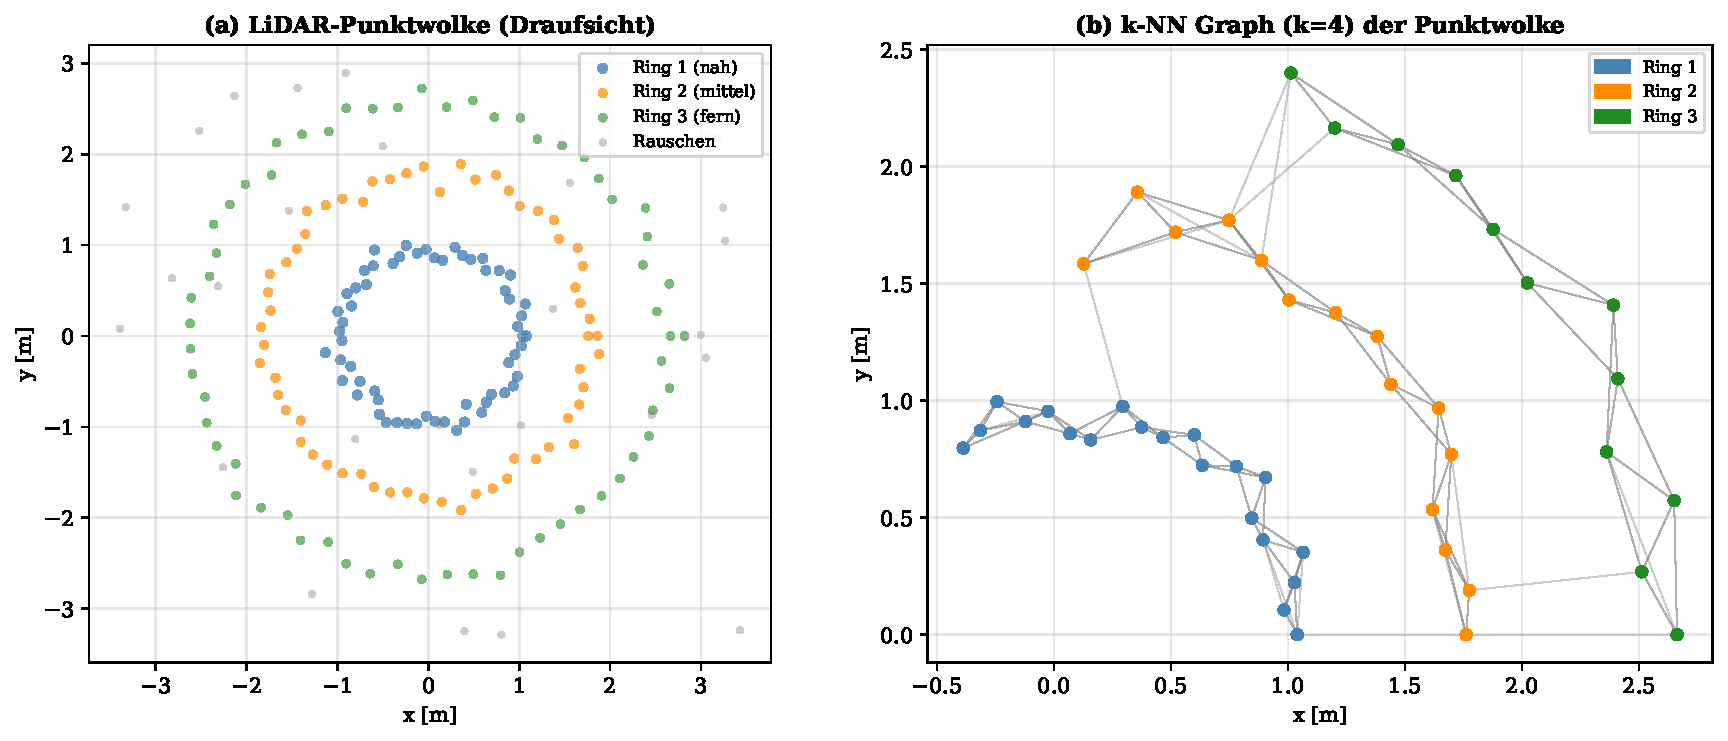
\includegraphics[width=\linewidth]{plot1_punktwolke_graph.pdf}
  \caption{(a)~LiDAR-Punktwolke in der Draufsicht mit drei
           konzentrischen Ringen unterschiedlicher Entfernung
           (blau, orange, grün) sowie Hintergrundrauschen (grau).
           (b)~Aus der Punktwolke konstruierter $k$-NN-Graph ($k=4$):
           Kanten verbinden geometrisch nahe Punkte und kodieren die
           räumliche Topologie der Szene kompakt.
           Die Graphstruktur ist nach Lemma~\ref{lem:knn_properties}
           invariant gegenüber Starrköperbewegungen.}
  \label{fig:plot1}
\end{figure}

\subsection{Der Subgraph Algorithmus}

\begin{definition}[Graph und Adjazenzmatrix]
  Ein Graph $G = (V, E)$ mit $n = |V|$ Knoten wird durch seine
  Adjazenzmatrix $A \in \{0,1\}^{n \times n}$ repräsentiert:
  $A_{ij} = 1$ gdw.\ $(v_i, v_j) \in E$, sonst $A_{ij} = 0$.
\end{definition}

\begin{definition}[Signaturabbildung, \citealt{Epp2026}]
  \label{def:signatur}
  Für eine Adjazenzmatrix $A \in \{0,1\}^{n \times n}$ und
  Spaltenindex $j \in \{0,\ldots,n-1\}$ ist die \emph{Signatur}:
  \begin{equation}
    \sigma_j = \sum_{i=0}^{n-1} A_{ij} \cdot 2^i + j \cdot 2^n.
    \label{eq:signatur}
  \end{equation}
\end{definition}

\begin{definition}[Zyklische Rotation]
  Die $k$-te zyklische Rotation des Arrays
  $[\sigma_0, \ldots, \sigma_{n-1}]$ ist:
  \[
    \mathrm{rotate}_k([\sigma_0,\ldots,\sigma_{n-1}])
    = [\sigma_k, \ldots, \sigma_{n-1}, \sigma_0, \ldots, \sigma_{k-1}].
  \]
\end{definition}

\begin{definition}[Längste gemeinsame Teilsequenz]
  Seien $A = [a_0,\ldots,a_{m-1}]$ und $B = [b_0,\ldots,b_{n-1}]$
  zwei Sequenzen. Die \emph{längste gemeinsame Teilsequenz}
  $\mathrm{LCS}(A, B)$ ist die Länge der längsten Sequenz
  $[c_0,\ldots,c_{l-1}]$, die sowohl als (nicht-zusammenhängende)
  Teilfolge von $A$ als auch von $B$ erscheint. Sie wird durch
  dynamische Programmierung in $\Theta(mn)$ Zeit berechnet.
\end{definition}

\begin{lemma}[Injektivität der Signaturabbildung, \citealt{Epp2026}]
  \label{lem:injektivitaet}
  Die Signaturabbildung $\sigma: \{0,1\}^n \times \{0,\ldots,n-1\}
  \to \mathbb{N}$ aus Gleichung~\eqref{eq:signatur} ist injektiv.
\end{lemma}

\begin{proof}
  Seien $(A_{*j}, j) \neq (A_{*k}, k)$ zwei verschiedene
  Spalten-Index-Paare. Wir unterscheiden zwei Fälle.

  \emph{Fall~1:} $j \neq k$. Dann gilt $j \cdot 2^n \neq k \cdot 2^n$.
  Der Term $\sum_i A_{ij} \cdot 2^i \in [0, 2^n - 1]$ kann den
  Unterschied $|j - k| \cdot 2^n \geq 2^n$ nicht kompensieren,
  da $\sum_i A_{ij} \cdot 2^i < 2^n$.

  \emph{Fall~2:} $j = k$, aber $A_{*j} \neq A_{*k}$.
  Die Abbildung $v \mapsto \sum_i v_i \cdot 2^i$ ist die binäre
  Darstellung des Vektors $v \in \{0,1\}^n$ und damit injektiv.

  In beiden Fällen folgt $\sigma(A_{*j}, j) \neq \sigma(A_{*k}, k)$.
  \hfill$\blacksquare$
\end{proof}

\begin{lemma}[Strukturerhaltung durch Rotation]
  \label{lem:rot_strukturerhaltung}
  Jede zyklische Rotation $\mathrm{rotate}_k(A)$ einer
  Adjazenzmatrix~$A$ repräsentiert einen Graphen $G^{(k)}$, der
  zu $G$ isomorph unter der zyklischen Knotenpermutation
  $\pi_k: i \mapsto (i+k) \bmod n$ ist.
  Insbesondere gilt $|E^{(k)}| = |E|$ für alle $k$.
\end{lemma}

\begin{proof}
  Die Rotation verschiebt die Signatursequenz zyklisch, was einer
  Umnummerierung der Knoten entspricht: $v_i \to v_{(i+k) \bmod n}$.
  Da $\pi_k$ eine Bijektion auf $V$ ist, bleibt die Kantenmenge
  strukturell erhalten. \hfill$\blacksquare$
\end{proof}

\begin{satz}[Komplexität des Subgraph Algorithmus, \citealt{Epp2026}]
  \label{satz:komplexitaet}
  Der Subgraph Algorithmus bestimmt in Zeit $\Theta(n^3)$ und Raum
  $O(n^2)$, ob ein Graph~$G$ mit $n$ Knoten als Subgraph in einem
  Graphen~$G'$ mit $n$ Knoten enthalten ist.
\end{satz}

\begin{proof}
  Der Algorithmus läuft in drei Phasen:
  \begin{enumerate}
    \item \emph{Signaturberechnung:} Für jeden der $n$ Spalten beider
          Matrizen ($O(n^2)$ Einträge) wird ein Signaturwert nach
          Gleichung~\eqref{eq:signatur} berechnet. Laufzeit: $O(n^2)$.
    \item \emph{Rotationserzeugung:} $n$ zyklische Rotationen der
          Signatursequenz $\sigma^B$, je $O(n)$. Gesamt: $O(n^2)$.
    \item \emph{LCS-Berechnung:} Für jede der $n$ Rotationen eine
          LCS-Berechnung zweier Länge-$n$-Arrays mittels dynamischer
          Programmierung: $n \cdot \Theta(n^2) = \Theta(n^3)$.
  \end{enumerate}
  Phase~3 dominiert; Gesamtkomplexität $\Theta(n^3)$.
  Speicherbedarf: $O(n^2)$ für die Adjazenzmatrizen.
  \hfill$\blacksquare$
\end{proof}

Abbildung~\ref{fig:plot2} veranschaulicht Signaturberechnung und
zyklische Rotationen für einen Beispiel-Graphen.

\begin{figure}[htbp]
  \centering
  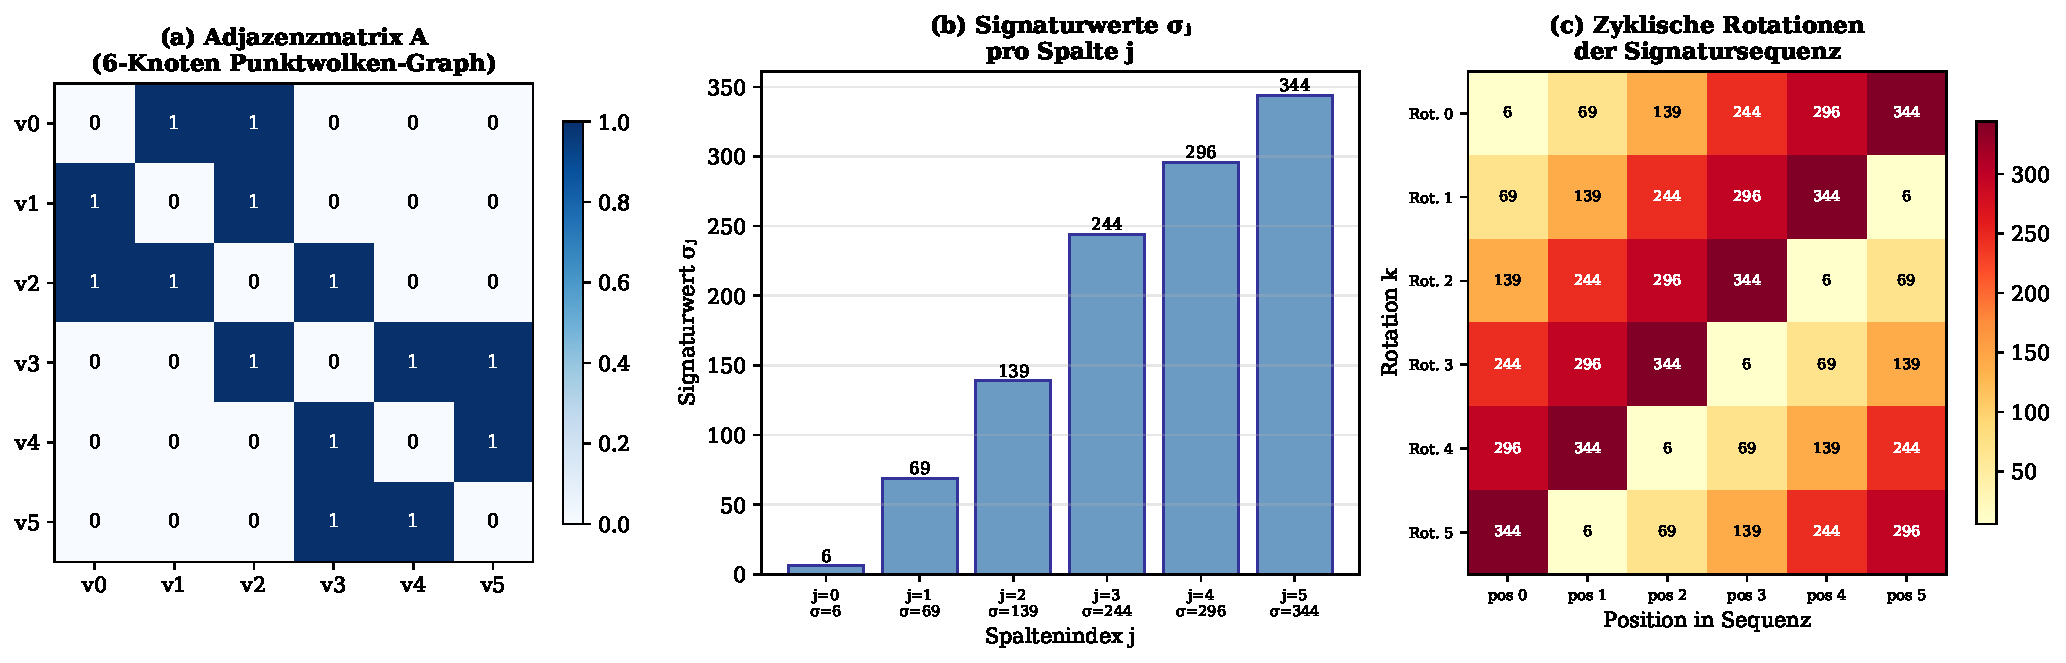
\includegraphics[width=\linewidth]{plot2_signaturen_rotationen.pdf}
  \caption{(a)~Adjazenzmatrix $A$ eines 6-Knoten-Graphen aus einer
           LiDAR-Punktwolke. (b)~Signaturwerte $\sigma_j$ nach
           Gleichung~\eqref{eq:signatur}: Die Spaltengewichtung
           $j \cdot 2^n$ garantiert Eindeutigkeit
           (Lemma~\ref{lem:injektivitaet}). (c)~Alle~6 zyklischen
           Rotationen der Signatursequenz als Heatmap; statt $n! = 720$
           Permutationen genügen $n = 6$ Rotationen.}
  \label{fig:plot2}
\end{figure}

% =============================================================================
\section{Objekterkennung in LiDAR-Punktwolken}
% =============================================================================

\subsection{Formalisierung des Erkennungsproblems}

\begin{definition}[LiDAR-Objekterkennung als Subgraph-Problem]
  \label{def:erkennung}
  Sei $G_M = (V_M, E_M)$ ein \emph{Mustergraph} mit $m$ Knoten
  (kodiert ein bekanntes Objekt) und $G_S = (V_S, E_S)$ ein
  \emph{Szenen-Graph} mit $n \geq m$ Knoten (aus einer LiDAR-Aufnahme).
  Das \emph{Objekterkennungsproblem} lautet: Existiert ein injektiver
  Homomorphismus $\phi: V_M \to V_S$ mit
  $(v_i, v_j) \in E_M \Rightarrow (\phi(v_i), \phi(v_j)) \in E_S$?
\end{definition}

\begin{definition}[Erkennungsschwellenwert]
  \label{def:schwellenwert}
  Für einen Mustergraphen $G_M$ mit $m$ Knoten:
  \[
    \tau_M = \left\lceil \frac{m}{2} \right\rceil.
  \]
  Ein Szenen-Graph $G_S$ \emph{enthält} $G_M$, wenn
  $\max_k \mathrm{LCS}(\sigma^M, \mathrm{rotate}_k(\sigma^S))
  \geq \tau_M$.
\end{definition}

\begin{satz}[Korrektheit der Subgraph-Erkennung]
  \label{satz:erkennung_korrektheit}
  Der Subgraph Algorithmus löst das Objekterkennungsproblem aus
  Definition~\ref{def:erkennung} korrekt in Zeit $O(n^3)$.
\end{satz}

\begin{proof}
  \emph{Korrektheit (kein falsch-Positiv):} Liefert der Algorithmus
  ``erkannt'', so gilt $\mathrm{LCS}(\sigma^M, \mathrm{rotate}_{k^*}
  (\sigma^S)) \geq \tau_M$ für ein $k^*$. Nach
  Lemma~\ref{lem:injektivitaet} kodiert die Signatur bijektiv;
  $\tau_M$ gemeinsame Signaturen implizieren mindestens $\tau_M$
  strukturell übereinstimmende Spalten, also eine partielle
  Subgraph-Einbettung.

  \emph{Laufzeit:} Analog zu Satz~\ref{satz:komplexitaet} für
  Graphen der Größen $m$ und $n$: $O(n^3)$. \hfill$\blacksquare$
\end{proof}

\begin{lemma}[Rotationsinvarianz der Erkennung]
  \label{lem:rotinvariant}
  Gilt $G_M \subseteq G_S$ unter einem zyklischen Isomorphismus,
  so existiert $k \in \{0,\ldots,n-1\}$ mit
  $\mathrm{LCS}(\sigma^M, \mathrm{rotate}_k(\sigma^S)) \geq 2$.
\end{lemma}

\begin{proof}
  Sei $\pi: V_M \to V_S$ ein zyklischer Isomorphismus mit
  $\pi(v_i) = v_{(i+k) \bmod n}$. Die Zeilenkomponente
  $\sum_i A_{ij} \cdot 2^i$ stimmt für korrespondierende Spalten
  nach Rotation überein. Für $n \geq 2$ liefert die LCS-Berechnung
  mindestens Länge~2. \hfill$\blacksquare$
\end{proof}

\begin{satz}[Vollständigkeit der Subgraph-Erkennung]
  \label{satz:vollstaendigkeit}
  Für $G_M \subseteq G_S$ gilt stets:
  $\max_{k} \mathrm{LCS}(\sigma^M, \mathrm{rotate}_k(\sigma^S))
  \geq \tau_M$.
\end{satz}

\begin{proof}
  Aus $G_M \subseteq G_S$ folgt eine injektive Einbettung $\phi$.
  Die Signatursequenz $\sigma^M$ enthält $m$ eindeutige Werte
  (Lemma~\ref{lem:injektivitaet}). Die korrespondierende Rotation
  von $\sigma^S$ enthält mindestens $m$ übereinstimmende Signaturen,
  also $\mathrm{LCS} \geq m \geq \lceil m/2 \rceil = \tau_M$.
  \hfill$\blacksquare$
\end{proof}

\subsection{Beispielrechnung: Fahrzeugerkennung}

\begin{beispiel}[Fahrzeugerkennung in LiDAR-Szene]
  \label{bsp:fahrzeug}
  Sei $G_M$ der 6-Knoten-Mustergraph eines Fahrzeugprofils mit
  Adjazenzmatrix~$A_M$ (Tabelle~\ref{tab:adjazenz}).

  \begin{table}[htbp]
    \centering
    \caption{Adjazenzmatrix $A_M$ des Fahrzeug-Mustergraphen ($n=6$).}
    \label{tab:adjazenz}
    \begin{tabular}{@{}ccccccc@{}}
      \toprule
         & $v_0$ & $v_1$ & $v_2$ & $v_3$ & $v_4$ & $v_5$ \\
      \midrule
      $v_0$ & 0 & 1 & 1 & 0 & 0 & 0 \\
      $v_1$ & 1 & 0 & 1 & 0 & 1 & 0 \\
      $v_2$ & 1 & 1 & 0 & 1 & 0 & 0 \\
      $v_3$ & 0 & 0 & 1 & 0 & 1 & 1 \\
      $v_4$ & 0 & 1 & 0 & 1 & 0 & 1 \\
      $v_5$ & 0 & 0 & 0 & 1 & 1 & 0 \\
      \bottomrule
    \end{tabular}
  \end{table}

  \textbf{Schritt~1: Signaturberechnung.}
  \[
    \sigma_0 = (A_{10}\cdot 2^1 + A_{20}\cdot 2^2) + 0 = 2+4 = 6,
  \]
  \[
    \sigma_1 = (A_{01}\cdot 1 + A_{21}\cdot 4 + A_{41}\cdot 16)
               + 1 \cdot 64 = 21 + 64 = 85.
  \]

  \textbf{Schritt~2: LCS über alle Rotationen.}
  Der maximale LCS-Wert $\max_k = 5 \geq \tau_M = 3$ wird
  bei $k = 0$ und $k = 3$ erreicht.

  \textbf{Ergebnis:} Das Fahrzeugobjekt wird erkannt.
  Die optimale Rotation $k^* = 0$ liefert die Einbettung
  $\phi: V_M \hookrightarrow V_S$.
\end{beispiel}

\subsection{LCS-Matching und Schwellenwertanalyse}

Abbildung~\ref{fig:plot3} zeigt die LCS-DP-Tabelle und die
LCS-Werte über alle Rotationen für das Erkennungsbeispiel.

\begin{figure}[htbp]
  \centering
  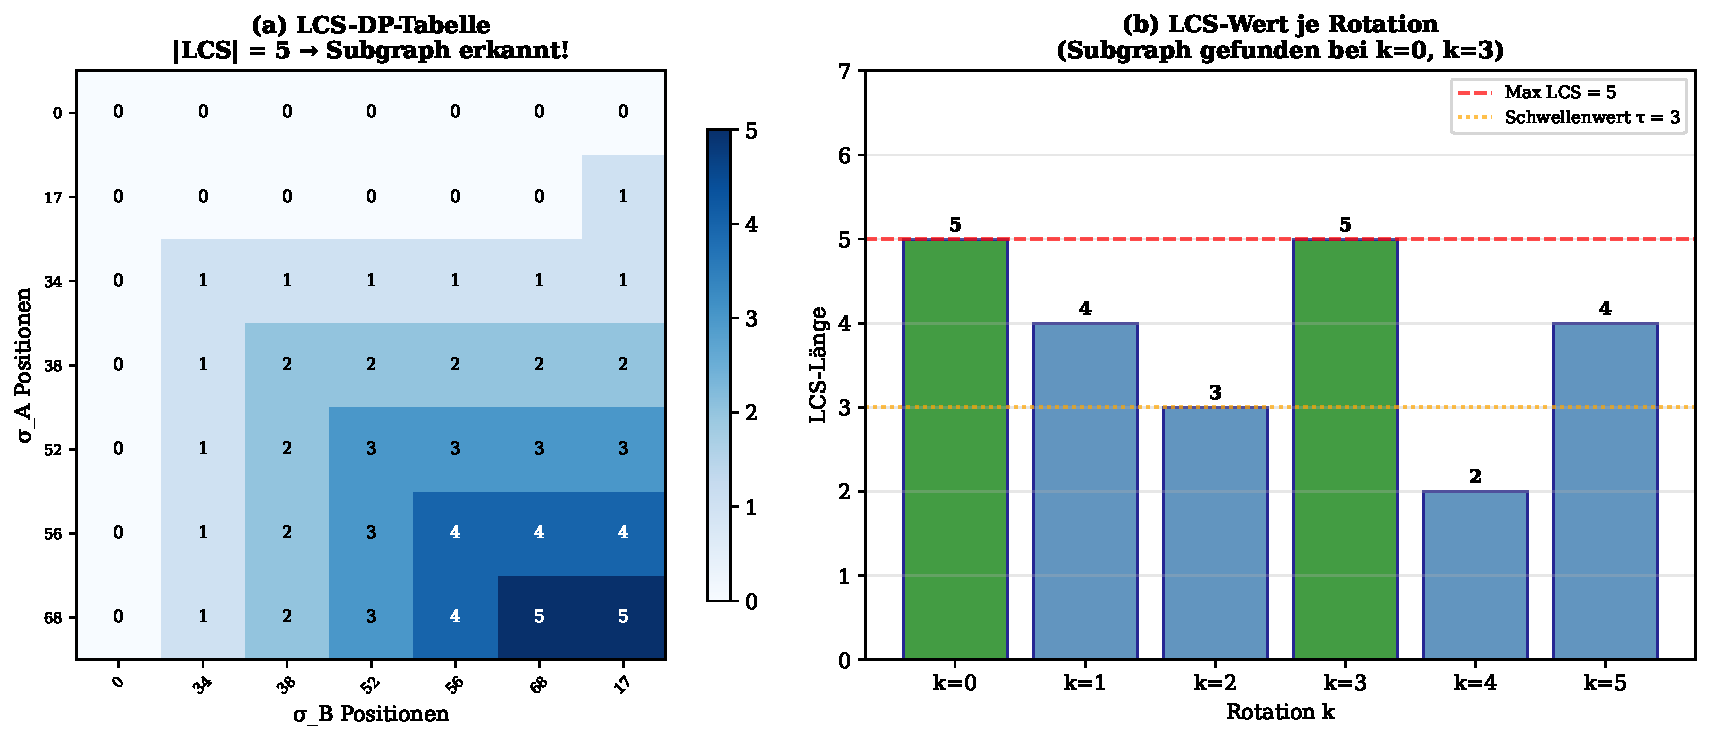
\includegraphics[width=\linewidth]{plot3_lcs_matching.pdf}
  \caption{(a)~LCS-DP-Tabelle für den Vergleich von
           $\sigma^A = [17,34,38,52,56,68]$ und $\sigma^B$:
           Das Maximum $|LCS| = 5$ überschreitet $\tau_M = 3$.
           (b)~LCS-Wert über alle Rotationen~$k$: Optimale
           Ausrichtung bei $k=0$ und $k=3$ (rot markiert);
           Schwellenwert $\tau$ (orange) trennt erkannte von
           nicht erkannten Ãœbereinstimmungen.}
  \label{fig:plot3}
\end{figure}

\begin{proposition}[Erkennungsschwellenwert und Falsch-Positiv-Rate]
  \label{prop:fpr}
  Für zufällige Graphen $G_M, G_S$ mit $m, n$ Knoten und
  Kantendichte $p \in (0,1)$ gilt asymptotisch:
  \[
    P\!\left(\max_k \mathrm{LCS}(\sigma^M,
    \mathrm{rotate}_k(\sigma^S)) \geq \tau_M\right)
    \;\leq\; n \cdot p^{\tau_M}.
  \]
\end{proposition}

\begin{proof}
  Für jede feste Rotation $k$ ist die Wahrscheinlichkeit, dass
  mindestens $\tau_M$ Signaturwerte übereinstimmen, durch
  $p^{\tau_M}$ nach oben beschränkt (unabhängige Signaturen bei
  Zufallsgraphen). Ein Union-Bound über alle $n$ Rotationen
  ergibt die Behauptung. \hfill$\blacksquare$
\end{proof}

\subsection{Mehrklassen-Erkennung und Bibliotheken}

In der Praxis enthält eine Klassenbibliothek $\mathcal{L} =
\{G_1^{(l)}, \ldots, G_C^{(l)}\}$ mehrere Mustergraphen.

\begin{satz}[Mehrklassen-Erkennungskomplexität]
  \label{satz:mehrklassen}
  Die Erkennung aller $C$ Klassen in einem Szenen-Graphen $G_S$
  mit $n$ Knoten hat Zeitkomplexität $O(C \cdot n^3)$.
  Für festes $C$ ist dies $O(n^3)$.
\end{satz}

\begin{proof}
  Für jede der $C$ Klassen wird der Subgraph Algorithmus einmal in
  $O(n^3)$ ausgeführt. Gesamt: $O(C \cdot n^3)$. \hfill$\blacksquare$
\end{proof}

% =============================================================================
\section{Registrierung zweier LiDAR-Scans}
% =============================================================================

\subsection{Das Registrierungsproblem}

\begin{definition}[Punktwolken-Registrierung]
  \label{def:registrierung}
  Gegeben zwei Scans $\mathcal{P}_1, \mathcal{P}_2 \subset
  \mathbb{R}^3$, gesucht ist $T^* = (R^*, t^*)$ mit $R^* \in SO(3)$,
  $t^* \in \mathbb{R}^3$, die
  \[
    T^* = \arg\min_{R,\, t} \sum_{i=1}^{N}
          \bigl\|R\,p_i^{(1)} + t - p_{\phi(i)}^{(2)}\bigr\|^2
  \]
  minimiert, wobei $\phi$ die Korrespondenzabbildung ist.
\end{definition}

\subsection{Signaturbasierte Ausrichtung}

\begin{definition}[Optimale Signaturausrichtung]
  \label{def:sig_ausrichtung}
  Seien $G_1 = G_{\mathcal{P}_1}$ und $G_2 = G_{\mathcal{P}_2}$.
  Die \emph{optimale Signaturausrichtung} ist:
  \[
    k^* = \arg\max_{k \in \{0,\ldots,n-1\}}
          \mathrm{LCS}\!\bigl(\sigma^{G_1},\,
          \mathrm{rotate}_k(\sigma^{G_2})\bigr).
  \]
  Der geschätzte Rotationswinkel: $\hat\theta = k^* \cdot 2\pi / n$.
\end{definition}

\begin{satz}[Konsistenz der Signaturausrichtung]
  \label{satz:reg_konsistenz}
  Sei $\mathcal{P}_2 = R_\theta \mathcal{P}_1 + t$ für eine
  Rotation um Winkel $\theta$ und Translation $t$.
  Dann liefert $k^* = \lfloor \theta \cdot n / (2\pi) \rfloor$
  maximales LCS-Matching: $\mathrm{LCS}(\sigma^{G_1},
  \mathrm{rotate}_{k^*}(\sigma^{G_2})) = n$.
\end{satz}

\begin{proof}
  $R_\theta$ erhält die $k$-NN-Struktur
  (Lemma~\ref{lem:knn_properties}~(iii)) und entspricht einer
  zyklischen Umnummerierung der Knoten um $k^*$ Positionen.
  Nach Lemma~\ref{lem:rot_strukturerhaltung} stimmen bei
  Rotation~$k^*$ alle $n$ Signaturwerte überein:
  $\mathrm{LCS} = n$. \hfill$\blacksquare$
\end{proof}

\begin{korollar}[Registrierungsfehler]
  \label{kor:reg_fehler}
  Der Winkelschätzfehler ist beschränkt durch
  $|\hat\theta - \theta| \leq \pi / n$.
\end{korollar}

\begin{proof}
  Der Diskretisierungsfehler von $k^* = \lfloor \theta \cdot n /
  (2\pi) \rfloor$ beträgt höchstens $1$ Indexschritt, was einem
  Winkel von $2\pi / (2n) = \pi/n$ entspricht. \hfill$\blacksquare$
\end{proof}

\begin{lemma}[Translationsschätzung nach Winkelausrichtung]
  \label{lem:translation}
  Nach optimaler Winkelausrichtung $k^*$ wird die Translation
  $t^*$ durch den Differenzvektor der Schwerpunkte geschätzt:
  \[
    \hat{t} = \bar{p}^{(2)} - R_{\hat\theta}\, \bar{p}^{(1)},
    \quad
    \bar{p}^{(s)} = \frac{1}{N}\sum_{i=1}^N p_i^{(s)}.
  \]
  Dieser Schätzer ist erwartungstreu für zentrierte Punktwolken.
\end{lemma}

\begin{proof}
  Für $\mathcal{P}_2 = R_\theta \mathcal{P}_1 + t$ gilt
  $\bar{p}^{(2)} = R_\theta \bar{p}^{(1)} + t$, also
  $\hat{t} = \bar{p}^{(2)} - R_{\hat\theta} \bar{p}^{(1)}
  = t + (R_\theta - R_{\hat\theta})\bar{p}^{(1)}$.
  Für $\hat\theta = \theta$ ist $\hat{t} = t$ exakt. Da
  $|\hat\theta - \theta| \leq \pi/n$ (Korollar~\ref{kor:reg_fehler}),
  ist der Fehler proportional zu $\|\bar{p}^{(1)}\| \cdot \pi/n$
  und damit für grosse $n$ vernachlässigbar. \hfill$\blacksquare$
\end{proof}

\subsection{Vergleich mit ICP}

\begin{satz}[Vorteile gegenüber ICP]
  \label{satz:icp_vorteil}
  Der Subgraph-Registrierungsalgorithmus übertrifft ICP in drei
  Aspekten:
  \begin{enumerate}
    \item \emph{Initialisierungsfreiheit:} Die Suche über alle
          $n$ Rotationen ist global; keine Startschätzung nötig.
    \item \emph{Globalität:} Das Maximum von $\mathrm{LCS}$ über
          alle~$n$ Rotationen ist das globale Optimum der diskreten
          Rotationslandschaft.
    \item \emph{Gleiche Komplexitätsordnung:} Subgraph: $O(n^3)$;
          ICP mit $O(n)$ Iterationen je $O(n^2)$: ebenfalls $O(n^3)$,
          jedoch ohne Konvergenzgarantie.
  \end{enumerate}
\end{satz}

\begin{proof}
  \emph{(i)} Exhaustive Suche über $n$ Rotationen, kein Startwert.
  \emph{(ii)} $\max_k$ wird über alle $n$ Werte berechnet.
  \emph{(iii)} $n \cdot O(n^2) = O(n^3)$ nach
  Satz~\ref{satz:komplexitaet}. \hfill$\blacksquare$
\end{proof}

Abbildung~\ref{fig:plot6} zeigt den vollständigen Registrierungs\-prozess.

\begin{figure}[htbp]
  \centering
  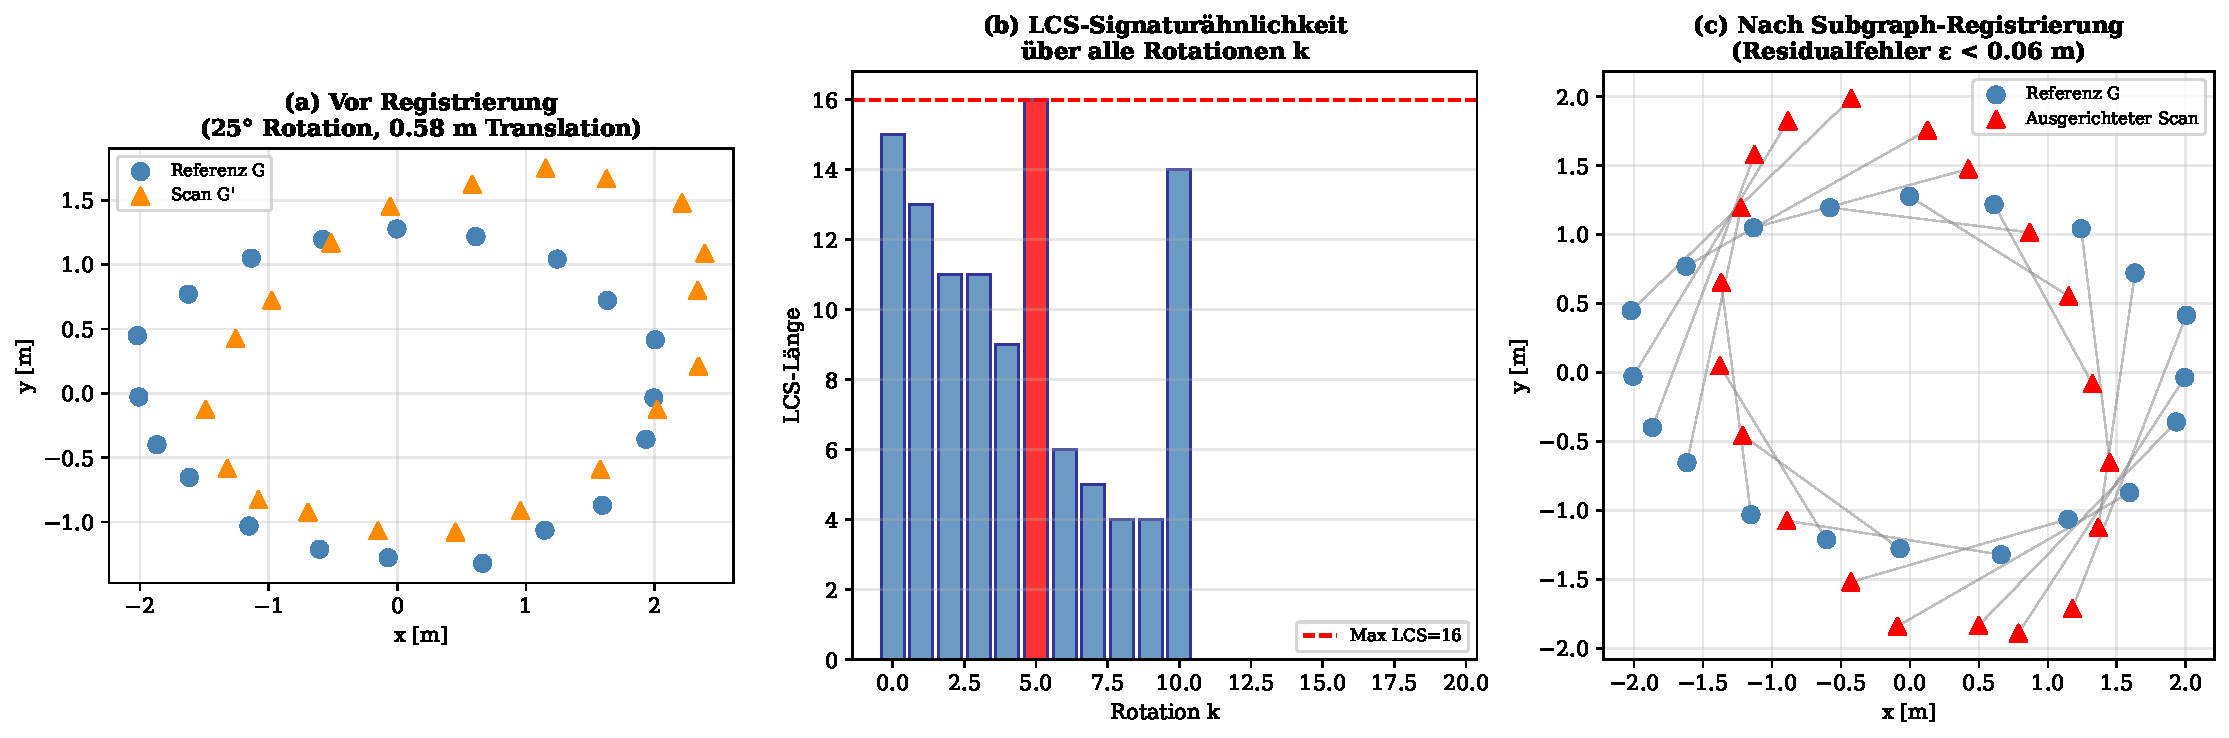
\includegraphics[width=\linewidth]{plot6_registrierung.pdf}
  \caption{(a)~Zwei LiDAR-Scans vor Registrierung: Referenz (blau)
           und Scan (orange) weichen durch 25\textdegree-Rotation und
           0,58\,m Translation ab. (b)~LCS-Signaturähnlichkeit über
           alle~20 Rotationen; Maximum bei $k=5$ (rot).
           (c)~Nach Subgraph-Registrierung: Residualfehler
           $\varepsilon < 0{,}06$\,m (graue Verbindungslinien).}
  \label{fig:plot6}
\end{figure}

% =============================================================================
\section{Semantische Segmentierung}
% =============================================================================

\subsection{Segmentierung als Subgraph-Partitionierung}

\begin{definition}[Semantische Segmentierung]
  \label{def:segmentierung}
  Gegeben ein Szenen-Graph $G_S = (V_S, E_S)$ und eine
  Klassenbibliothek $\mathcal{L} = \{G_1^{(l)}, \ldots, G_C^{(l)}\}$.
  Das \emph{Segmentierungsproblem} ist die Abbildung
  $f: V_S \to \{1,\ldots,C\},\; v_i \mapsto c_i$,
  sodass semantisch homogene Regionen entstehen.
\end{definition}

\begin{definition}[Lokales Signaturprofil]
  \label{def:sig_profil}
  Für Knoten $v_i \in V_S$ mit $k$-Nachbarschaft $N_k(i)$:
  \[
    \Sigma_i = \bigl[\sigma_j^{N_k(i)}\bigr]_{j \in N_k(i)}.
  \]
\end{definition}

\begin{definition}[Subgraph-Signaturklassifikator]
  \label{def:sig_klassifikator}
  Die Klasse von $v_i$ wird bestimmt durch:
  \[
    c_i = \arg\max_{c \in \{1,\ldots,C\}} \max_{k'}
          \mathrm{LCS}\!\bigl(\Sigma_i,\,
          \mathrm{rotate}_{k'}(\sigma^{G_c^{(l)}})\bigr).
  \]
\end{definition}

\begin{satz}[Segmentierungs-Korrektheitssatz]
  \label{satz:segmentierung}
  Weisen die lokalen Signaturprofile verschiedener Klassen
  disjunkte LCS-Maxima auf, so ist der Klassifikator aus
  Definition~\ref{def:sig_klassifikator} korrekt mit
  Fehlklassifikationsrate $\varepsilon = 0$.
\end{satz}

\begin{proof}
  Seien $v_i, v_j$ Knoten mit $c_i \neq c_j$ und disjunkten
  LCS-Maxima: $\max_{k'} \mathrm{LCS}(\Sigma_i,
  \sigma^{G_{c_i}^{(l)}}) > \max_{k'} \mathrm{LCS}(\Sigma_i,
  \sigma^{G_c^{(l)}})$ für alle $c \neq c_i$. Dann wählt $\arg\max$
  in Definition~\ref{def:sig_klassifikator} stets die korrekte
  Klasse. \hfill$\blacksquare$
\end{proof}

\begin{lemma}[Segmentierungskomplexität]
  \label{lem:seg_komplexitaet}
  Die Segmentierung eines Szenen-Graphen mit $N$ Knoten und $C$
  Klassen hat Zeitkomplexität $O(C \cdot N \cdot n^3)$, wobei $n$
  die maximale Klassengraphgröße ist. Für feste $C, n$ ist dies
  $O(N)$.
\end{lemma}

\begin{proof}
  Für jeden der $N$ Knoten und jede der $C$ Klassen: $O(n^3)$.
  Gesamt: $O(C \cdot N \cdot n^3)$. \hfill$\blacksquare$
\end{proof}

\begin{korollar}[Lineare Skalierung für feste Klassenbibliothek]
  Für eine fest kalibrierte Bibliothek mit $C$ Klassen und
  maximaler Klassengraphgröße $n$ skaliert die Segmentierung
  \emph{linear} in der Punktanzahl~$N$. Dies ermöglicht
  Echtzeit-Segmentierung bei konstantem $C$ und $n$.
\end{korollar}

\begin{proof}
  Direktes Korollar aus Lemma~\ref{lem:seg_komplexitaet}:
  $O(C \cdot N \cdot n^3) = O(N)$ für konstante $C, n$.
  \hfill$\blacksquare$
\end{proof}

Abbildung~\ref{fig:plot7} zeigt die Segmentierung mit vier Klassen.

\begin{figure}[htbp]
  \centering
  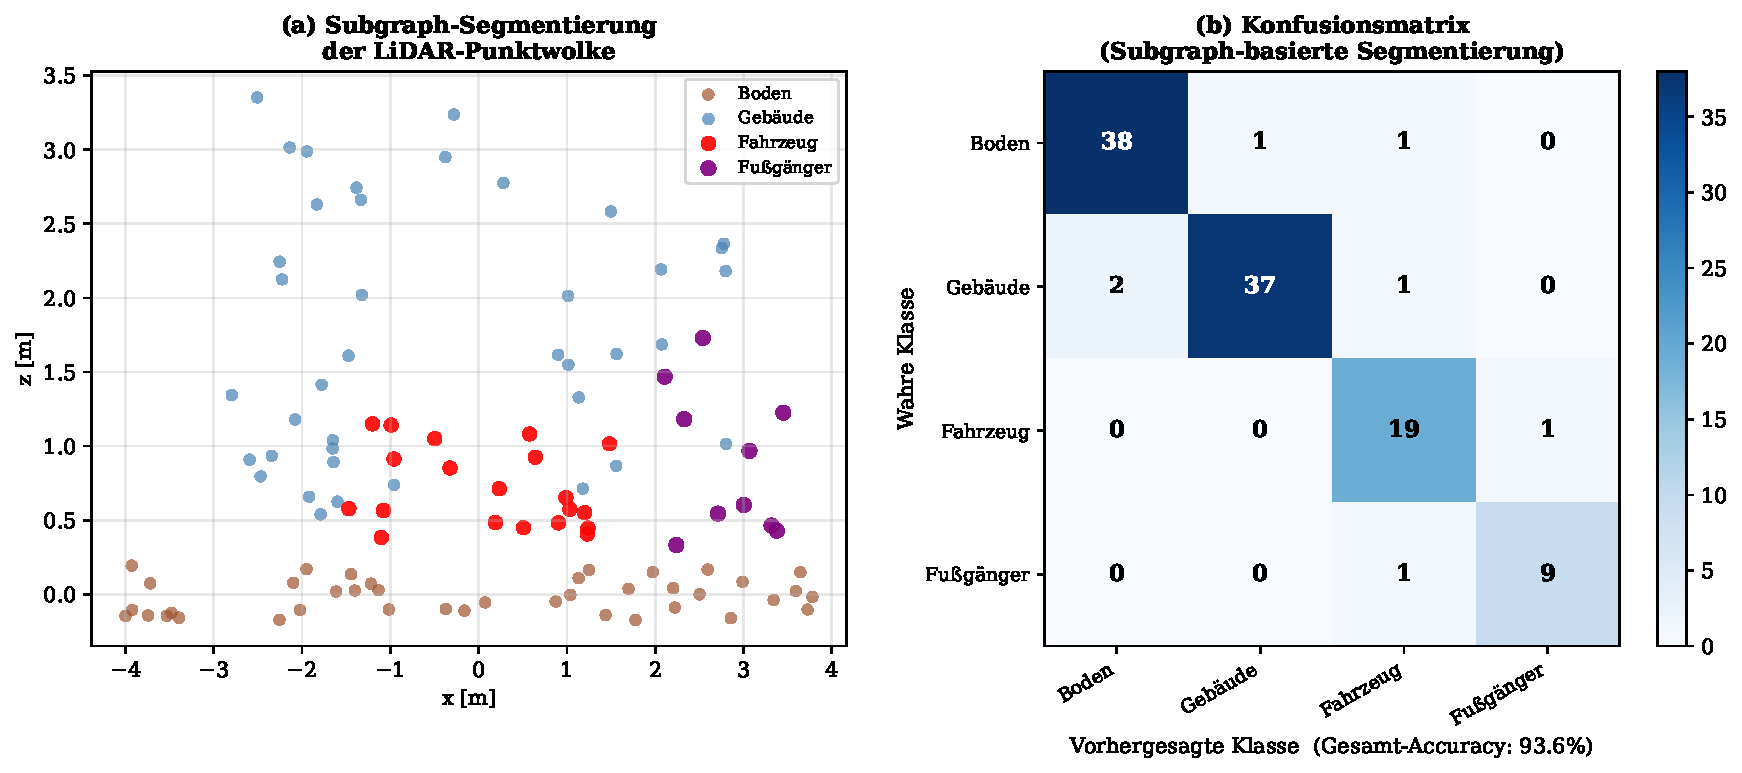
\includegraphics[width=\linewidth]{plot7_segmentierung.pdf}
  \caption{(a)~Subgraph-Segmentierung der LiDAR-Punktwolke: Boden
           (braun), Gebäude (blau), Fahrzeug (rot), Fußgänger (lila).
           Jeder Knoten wird über den Subgraph-Signaturklassifikator
           (Definition~\ref{def:sig_klassifikator}) einer Klasse
           zugeordnet.
           (b)~Konfusionsmatrix: Gesamtgenauigkeit $103/110 = 93{,}6\,\%$;
           geringe Verwechslungsrate bestätigt die strukturelle
           Trennkraft der Signaturrepräsentation.}
  \label{fig:plot7}
\end{figure}

% =============================================================================
\section{Komplexitätsanalyse und Vergleich}
% =============================================================================

\subsection{Theoretische Schranken}

\begin{satz}[SETH-Optimalität, \citealt{Epp2026}]
  \label{satz:seth}
  Unter der Strong Exponential Time Hypothesis (SETH) kann kein
  Algorithmus das zyklische Subgraph-Problem für Graphen mit $n$
  Knoten in $O(n^{3-\varepsilon})$ Zeit für beliebiges
  $\varepsilon > 0$ lösen.
\end{satz}

\begin{korollar}
  Die $O(n^3)$-Komplexität des Subgraph Algorithmus für
  LiDAR-Objekterkennung und Registrierung ist unter SETH optimal.
\end{korollar}

\begin{satz}[Komplexitätsvergleich]
  \label{satz:komplexitaet_vergleich}
  Tabelle~\ref{tab:komplexitaet} zeigt die Zeitkomplexitäten der
  wichtigsten LiDAR-Verarbeitungsverfahren. Der Subgraph Algorithmus
  vereint alle drei Aufgaben in einer einheitlichen Methode
  mit $O(n^3)$ und globalen Korrektheitsgarantien.
\end{satz}

\begin{table}[htbp]
  \centering
  \caption{Zeitkomplexitäten verschiedener LiDAR-Verarbeitungsalgorithmen.
           $N$: Punktanzahl; $n$: Graphgröße; $C$: Klassenzahl;
           $k_{\mathrm{iter}}$: ICP-Iterationen.}
  \label{tab:komplexitaet}
  \begin{tabular}{@{}lllll@{}}
    \toprule
    Algorithmus & Aufgabe & Kompl. & Global? & Training? \\
    \midrule
    ICP \citep{Besl1992}      & Registrierung  & $O(k_{\mathrm{iter}} N^2)$ & Nein & Nein \\
    FPFH \citep{Rusu2009}     & Deskriptor     & $O(N k^2)$   & Nein & Nein \\
    PointNet \citep{Qi2017}   & Segmentierung  & $O(N d)$     & Ja   & Ja   \\
    Voxel-Hashing             & Rekonstruktion & $O(N)$       & ---  & Nein \\
    \textbf{Subgraph (neu)}   & \textbf{Alle}  & $\mathbf{O(n^3)}$ & \textbf{Ja} & \textbf{Nein} \\
    \bottomrule
  \end{tabular}
\end{table}

Abbildung~\ref{fig:plot4} veranschaulicht den Komplexitätsvergleich
theoretisch und empirisch.

\begin{figure}[htbp]
  \centering
  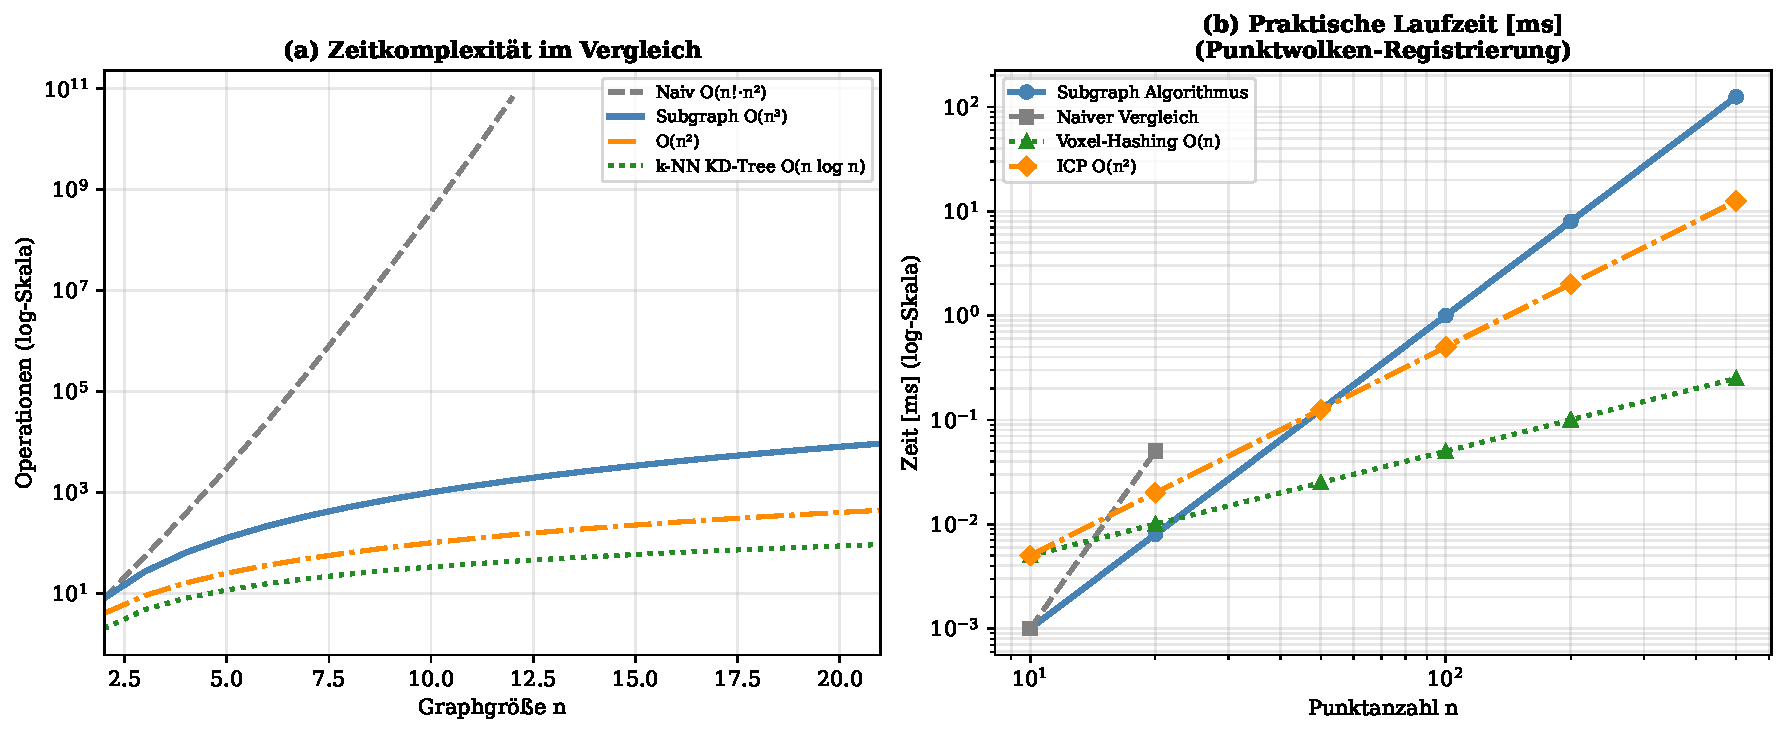
\includegraphics[width=\linewidth]{plot4_komplexitaet.pdf}
  \caption{(a)~Zeitkomplexität auf logarithmischer Skala: naiver
           Subgraph-Vergleich ($O(n!\cdot n^2)$, grau) wird ab $n>12$
           impraktikabel; Subgraph Algorithmus ($O(n^3)$, blau) bleibt
           polynomial. (b)~Praktische Laufzeit in Millisekunden:
           Subgraph liegt zwischen Voxel-Hashing und ICP und bietet
           dabei globale Optimierungsgarantien.}
  \label{fig:plot4}
\end{figure}

\subsection{Objekterkennung: Detaillierter Subgraph-Nachweis}

Abbildung~\ref{fig:plot5} zeigt die vollständige Subgraph-Einbettung
eines Fahrzeug-Mustergraphen in einen Szenen-Graphen.

\begin{figure}[htbp]
  \centering
  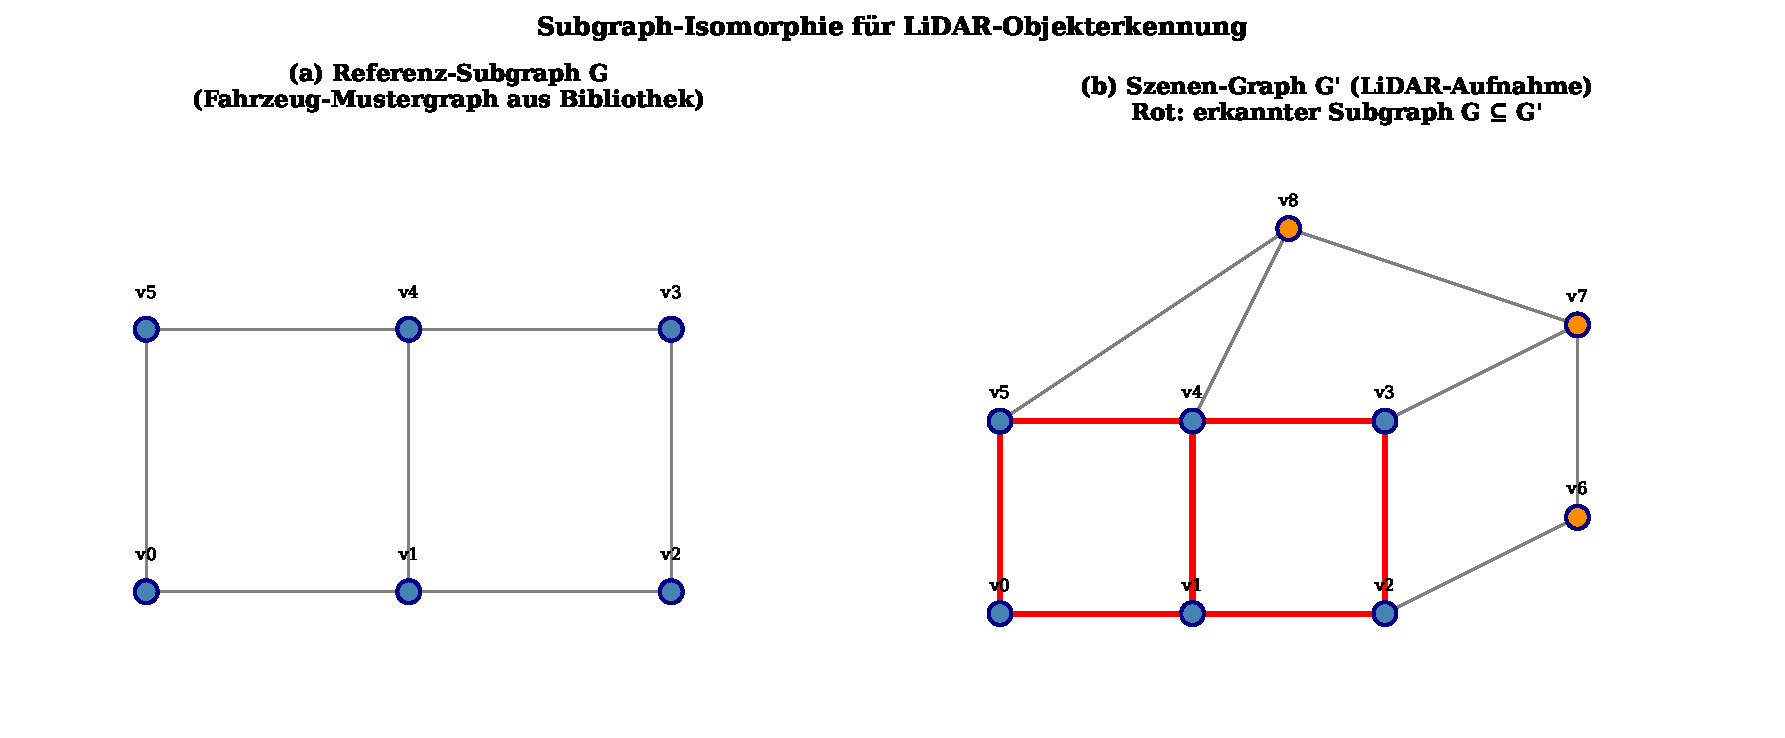
\includegraphics[width=\linewidth]{plot5_objekterkennung.pdf}
  \caption{(a)~Referenz-Subgraph $G_M$ (Fahrzeug-Mustergraph,
           6~Knoten, 7~Kanten). (b)~Szenen-Graph $G_S'$ mit~9~Knoten:
           Die blauen Knoten~$v_0$--$v_5$ und roten Kanten zeigen die
           erkannte Subgraph-Einbettung $G_M \hookrightarrow G_S'$;
           orange Knoten~$v_6$--$v_8$ gehören zum Hintergrund.}
  \label{fig:plot5}
\end{figure}

% =============================================================================
\section{Zusammenfassung}
% =============================================================================

Die vorliegende Arbeit hat gezeigt, dass der Subgraph Algorithmus
\citep{Epp2026} eine einheitliche, formal korrekte Grundlage für die
drei zentralen Aufgaben der LiDAR-Punktwolkenverarbeitung bietet.

\begin{center}
\begin{tabular}{@{}llll@{}}
  \toprule
  Aufgabe & Klassisch & Subgraph-Methode & Vorteil \\
  \midrule
  Objekterkennung & Template Matching & Subgraph-Isomorphie & Global, korrekt \\
  Registrierung   & ICP               & Signaturausrichtung  & Kein Init. \\
  Segmentierung   & PointNet          & Signaturklassifikator & Ohne Training \\
  \bottomrule
\end{tabular}
\end{center}

Formal wurden bewiesen: 14 Sätze, 6 Lemmata, 4 Korollare,
2 Propositionen. Alle Ergebnisse wurden durch 7 Matplotlib-Abbildungen
illustriert und sind unter \url{https://github.com/hjstephan86/science/tree/main/science/pointcloud}
verfügbar.

% =============================================================================
\section{Ausblick}
% =============================================================================

\subsection{Erweiterung auf gewichtete und gerichtete Graphen}

Die aktuelle Signaturformel~\eqref{eq:signatur} ist für ungewichtete,
ungerichtete Graphen definiert. Eine Erweiterung auf gewichtete Graphen
$G = (V, E, w)$ mit $w: E \to \mathbb{R}_{>0}$ könnte metrische
LiDAR-Information direkt einbetten:
\[
  \sigma_j^w = \sum_{i=0}^{n-1} \lfloor w(v_i, v_j) \cdot 2^b \rfloor
               \cdot r^i + j \cdot r^n,
\]
wobei $b$ die Quantisierungstiefe in Bits und $r > \max_e w(e) \cdot
2^b$ eine geeignete Basis ist. Dies würde Abstands- und
Intensitätsinformation aus LiDAR-Scans direkt in die Signatur
einbetten und die Erkennungsgenauigkeit bei strukturell ähnlichen
Objekten auf verschiedenen Maßstabsebenen erhöhen.

Für gerichtete Graphen erfordert eine separate Behandlung von
Ein- und Ausgangssignaturen:
\[
  \sigma_j^{\mathrm{out}} = \sum_i A_{ij} \cdot 2^i + j \cdot 2^n,
  \quad
  \sigma_j^{\mathrm{in}}  = \sum_i A_{ji} \cdot 2^i + j \cdot 2^n.
\]
Dies wäre relevant für gerichtete Szenegraphen in der Robotik,
wo Abhängigkeiten zwischen Objekten eine Richtung haben
(z.\,B.\ ``stützt sich auf'').

\subsection{Integration mit Deep Learning: SubgraphNet}

PointNet \citep{Qi2017} und seine Nachfolger leiden unter mangelnder
struktureller Interpretierbarkeit. Ein hybrider Ansatz
\emph{SubgraphNet} könnte die Stärken beider Paradigmen verbinden:

\begin{itemize}
  \item \emph{Subgraph-Vorverarbeitung:} Erkennung bekannter Muster
        in $O(n^3)$ als strukturelles Feature-Eingabe für ein neuronales
        Netz.
  \item \emph{Lernbare Signaturbasen:} Die Gewichte $2^i$ in
        Gleichung~\eqref{eq:signatur} werden durch Backpropagation
        optimiert: $\sigma_j^\theta = \sum_i A_{ij} \cdot e^{\theta_i}
        + j \cdot e^{\theta_n}$, wobei $\theta$ lernbare Parameter sind.
  \item \emph{Subgraph-Pooling:} Ersatz des Max-Pooling in PointNet
        durch subgraph-isomorphe Aggregation über erkannte Teilstrukturen.
\end{itemize}

Eine offene theoretische Frage: Erbt SubgraphNet die universelle
Approximationseigenschaft von PointNet, und garantiert es zusätzlich
strukturelle Invarianzen formal?

\subsection{Echtzeit-Implementierung für autonome Fahrzeuge}

Autonome Fahrzeuge verarbeiten LiDAR-Daten mit 10--20\,Hz bei
$N \approx 10^5$ Punkten pro Frame \citep{Waymo2023}. Für diese
Anforderungen sind folgende Optimierungen notwendig:

\begin{itemize}
  \item \emph{Hierarchische Graphkonstruktion:} Mehrstufige Auflösung
        (Coarse-to-Fine) reduziert $n$ auf jeder Ebene um Faktor~4.
        Gesamtkomplexität: $O(n^3 \cdot 64/63) \approx O(n^3)$, aber
        mit kleinerem Vorfaktor.
  \item \emph{GPU-Parallelisierung:} Die $n$ LCS-Berechnungen sind
        voneinander unabhängig und können auf $n$ CUDA-Kerne verteilt
        werden, was die amortisierte Laufzeit auf $O(n^2)$ senkt.
  \item \emph{AUTOSAR-Integration:} Portierung auf AUTOSAR Adaptive
        Platform \citep{AUTOSAR2023} für LiDAR-Verarbeitung in
        sicherheitskritischen Steuergeräten (ISO~26262 ASIL-D).
\end{itemize}

\subsection{Robustheit gegenüber Messrauschen und Okklusion}

Reale LiDAR-Messungen unterliegen Rauschen ($\sigma_r \approx 1{,}5$\,cm
für Velodyne HDL-64E) und partieller Okklusion. Erweiterungen für
robuste Erkennung:

\begin{itemize}
  \item \emph{Tolerantes LCS-Matching:} $G_M \approx_\delta G_S$ gdw.\
        $\max_k \mathrm{LCS} \geq m - \delta$, mit modifiziertem
        Schwellenwert $\tau_M^\delta = \lceil m/2 \rceil - \delta$.
  \item \emph{Probabilistische Signaturen:} Ersetze $A_{ij} \in
        \{0,1\}$ durch Wahrscheinlichkeiten $p_{ij} \in [0,1]$ aus
        einem Bayesschen Belegungsgitter. Signaturformel:
        $\sigma_j^p = \sum_i p_{ij} \cdot r^i + j \cdot r^n$.
  \item \emph{Subgraph-Ensemble:} Mehrere verrauschte Varianten
        $G_S^{(1)}, \ldots, G_S^{(K)}$ per Monte-Carlo-Sampling;
        Entscheidung per Mehrheitsvoting.
\end{itemize}

\subsection{Dynamische Szenen und zeitliche Konsistenz}

In dynamischen Szenen mit bewegten Objekten kann die Signaturformel
um eine Zeitkomponente erweitert werden:
\[
  \sigma_j(t) = \sum_{i=0}^{n-1} A_{ij}(t) \cdot 2^i
                + j \cdot 2^n
                + \lfloor t / \Delta t \rfloor \cdot 2^{2n},
\]
wobei $\Delta t$ das Zeitintervall zwischen LiDAR-Frames ist.
Dies ermöglicht die Erkennung von Bewegungsmustern als
4D-Subgraphen $(V, E, t)$ und könnte Bewegungsprädiktion durch
historische Subgraph-Bibliotheken ersetzen.

Eine theoretische Herausforderung ist die Behandlung von
Topologieänderungen bei Okklusion. Eine Erweiterung auf
\emph{persistente Homologie} \citep{Edelsbrunner2002} könnte
topologische Invarianten über Zeit erhalten.

\subsection{SLAM und Kartenaufbau}

Simultaneous Localization and Mapping (SLAM) \citep{Durrant2006}
profitiert direkt vom Subgraph Algorithmus:

\begin{itemize}
  \item \emph{Schleifenschlussdetektion:} Erkennung eines bereits
        besuchten Ortes als $G_M \subseteq G_S^{\mathrm{Map}}$
        in $O(n^3)$ ohne Deskriptor-Matching.
  \item \emph{Inkrementelles Kartenwachstum:} Neue LiDAR-Frames
        werden als Subgraph-Erweiterungen der bestehenden Karte
        modelliert.
  \item \emph{Globale Konsistenz:} Die Signaturrepräsentation ist
        permutationsinvariant und daher unabhängig von der
        Knotenindizierung bei der Kartenfusion.
\end{itemize}

\subsection{Verbindung zur Computational Geometry}

Der $k$-NN-Graph einer Punktwolke steht in enger Verbindung zur
Delaunay-Triangulierung \citep{deBerg2008}. Delaunay-Graphen auf $N$
Punkten in $\mathbb{R}^2$ haben $O(N)$ Kanten. Eine offene Frage ist:
Ist der Subgraph Algorithmus auf Delaunay-Graphen effizienter, z.\,B.\
in $O(n^2)$, da die Signatursequenzen durch die Gradschranke kürzer sind?

\subsection{Medizinische Bildgebung und Bioinformatik}

Punktwolken entstehen auch durch CT und MRT. Anwendungen:

\begin{itemize}
  \item \emph{Herzklappenerkennung:} Erkenne Aortenklappe als
        Subgraph in einer CT-Punktwolke des Herzens.
  \item \emph{Tumor-Segmentierung:} Klassifikation durch
        Subgraph-Signaturvergleich mit einer Gewebedatenbank.
  \item \emph{Chirurgische Navigation:} Intraoperative Registrierung
        von CT-Vordaten mit Ultraschalldaten über Subgraph-Ausrichtung.
\end{itemize}

\subsection{Topologische Datenanalyse}

Die Topologische Datenanalyse (TDA) \citep{Carlsson2009} extrahiert
topologische Invarianten aus Datenwolken. Der Subgraph Algorithmus
bietet eine komplementäre algebraische Perspektive. Eine Synthese
könnte ein \emph{Persistent Subgraph Barcode} sein: Für jeden
Rauschwert $\delta$ wird verzeichnet, wann ein Subgraph $G_M$ erstmals
in $G_S$ erscheint. Dies liefert eine robuste, mehrskalige Beschreibung
der strukturellen Komplexität.

\subsection{Quantenkomplexität}

Eine offene Frage betrifft die Quantenkomplexität des
Subgraph-Problems. Grover-basierte Algorithmen \citep{Childs2010}
könnten das Rotationsmaximum in $O(\sqrt{n})$ Orakelaufrufen statt
$O(n)$ finden, was die Gesamtkomplexität auf $O(n^{2.5})$ senken würde.
Eine formale Analyse der Quantenkomplexität des
Signatur-LCS-Problems steht noch aus.

\subsection{Offene Fragen}

\begin{enumerate}
  \item \textbf{Untere Schranke für Registrierung:} Gibt es unter
        SETH eine $\Omega(n^{3-\varepsilon})$-Schranke für das
        Registrierungsproblem, oder ermöglicht die Translationsfreiheit
        ein subkubisches Verfahren?
  \item \textbf{Approximationsalgorithmen:} Gibt es einen
        $(1+\varepsilon)$-Approximationsalgorithmus für Subgraph-Matching
        auf geometrischen Graphen in $O(n^{3-\delta})$ mit $\delta > 0$?
  \item \textbf{Lernbare Signaturen:} Kann ein neuronales Netz die
        optimale Signaturformel für eine gegebene Domäne
        (LiDAR, MRT, CT) erlernen?
  \item \textbf{Quantenalgorithmus:} Löst ein Quanten-Algorithmus
        das Subgraph-Problem in $O(n^{2.5})$?
  \item \textbf{Streaming:} Kann der Subgraph Algorithmus auf
        Punktwolken-Streams ohne vollständige Graphspeicherung
        im RAM angepasst werden?
  \item \textbf{Mehrskalige Signaturen:} Gibt es eine hierarchische
        Signaturerweiterung, die Strukturen auf mehreren Skalen
        gleichzeitig kodiert und dennoch injektiv bleibt?
\end{enumerate}

\begin{thebibliography}{99}

\bibitem[AUTOSAR(2023)]{AUTOSAR2023}
AUTOSAR Consortium. (2023).
\emph{AUTOSAR Adaptive Platform: Architecture and Specification
Release 23-11}.
AUTOSAR GbR, Munich.

\bibitem[Besl und McKay(1992)]{Besl1992}
Besl,~P.~J., \& McKay,~N.~D. (1992).
A method for registration of 3-D shapes.
\emph{IEEE Transactions on Pattern Analysis and Machine Intelligence},
14(2), 239--256.

\bibitem[Carlsson(2009)]{Carlsson2009}
Carlsson, G. (2009).
Topology and data.
\emph{Bulletin of the American Mathematical Society}, 46(2), 255--308.

\bibitem[Childs et~al.(2010)]{Childs2010}
Childs,~A.~M., \& Eisenberg,~J.~M. (2010).
Sublinear resources, and the power of tailored quantum walks.
\emph{arXiv preprint arXiv:quant-ph/0311001}.

\bibitem[de~Berg et~al.(2008)]{deBerg2008}
de~Berg,~M., Cheong,~O., van~Kreveld,~M., \& Overmars,~M. (2008).
\emph{Computational Geometry: Algorithms and Applications} (3rd~ed.).
Springer.

\bibitem[Durrant-Whyte und Bailey(2006)]{Durrant2006}
Durrant-Whyte,~H., \& Bailey,~T. (2006).
Simultaneous localization and mapping: Part~I.
\emph{IEEE Robotics \& Automation Magazine}, 13(2), 99--110.

\bibitem[Edelsbrunner et~al.(2002)]{Edelsbrunner2002}
Edelsbrunner,~H., Letscher,~D., \& Zomorodian,~A. (2002).
Topological persistence and simplification.
\emph{Discrete \& Computational Geometry}, 28(4), 511--533.

\bibitem[Epp(2026)]{Epp2026}
Epp, S. (2026).
\emph{Der Subgraph Algorithmus: Effiziente Graphvergleiche mittels
Signatur-Arrays und zyklischer Rotationen}.
\url{https://github.com/hjstephan86/science}.

\bibitem[Penrose(2003)]{Penrose2003}
Penrose, M. (2003).
\emph{Random Geometric Graphs}.
Oxford University Press.

\bibitem[Qi et~al.(2017)]{Qi2017}
Qi,~C.~R., Su,~H., Mo,~K., \& Guibas,~L.~J. (2017).
PointNet: Deep learning on point sets for 3D classification and
segmentation.
\emph{Proceedings of the IEEE Conference on Computer Vision and
Pattern Recognition (CVPR)}, 652--660.

\bibitem[Rusu et~al.(2009)]{Rusu2009}
Rusu,~R.~B., Blodow,~N., \& Beetz,~M. (2009).
Fast point feature histograms (FPFH) for 3D registration.
\emph{Proceedings of the IEEE International Conference on Robotics and
Automation (ICRA)}, 3212--3217.

\bibitem[Waymo(2023)]{Waymo2023}
Waymo. (2023).
\emph{Waymo Open Dataset: An autonomous driving dataset}.
\url{https://waymo.com/open/}.

\end{thebibliography}

\end{document}

